\documentclass[11pt,french,a4paper]{article}

\usepackage[utf8]{inputenc}
\usepackage[T1]{fontenc}

\usepackage[french]{babel}
\usepackage[a4paper,fancysections]{polytechnique}
\usepackage[hidelinks]{hyperref}
\usepackage{amsmath}
\usepackage{url}
\usepackage{graphicx}
\usepackage{shortvrb}
\MakeShortVerb{\|}

\title{Rapport de projet INF441}
\subtitle{Les liens dansants}
\author{Antoine \bsc{Berthier}\\ Denis \bsc{Merigoux}}
\date{Mardi 2 juin 2015}

\begin{document}

\maketitle

\section{Organisation du travail}

\paragraph{GitHub} Afin de coordonner nos efforts et assurer un suivi optimal de notre projet, nous avons utilisé un contrôle de version Git collaboratif. Notre projet est donc également disponible à l'adresse \url{https://github.com/denismerigoux/ProjetINF441}.

\paragraph{Contributions et organisation} Nous nous sommes répartis le travail comme il suit :
\begin{itemize}
	\item Denis a établi les modèles de données, écrit l'algorithme et s'est occupé des aspects plus théoriques du problème ;
	\item Antoine a réalisé les méthodes d'entrée/sortie et de création d'un objet utilisable par l'algorithme à partir de l'entrée imposée.
\end{itemize}

Toutes les fichiers source se trouvent dans le dossier |src| conformément à l'énoncé. On distingue trois catégories dans ces fichiers.

\paragraph{Algorithme} D'abord les fichiers liés à l'algorithme DLX et à la structure de données permettant de le réaliser :
\begin{itemize}
	\item |LinkObject|, classe abstraite modélisant implémentées par tous les objects ci-dessous ;
	\item |DataObject| qui modélise les 1 dans les matrices EMC ;
	\item |ColmunObject| qui modélise les en-têtes de colonnes ;
	\item |RootObject| pour l'objet \emph{root} décrit dans l'article ;
	\item |LinkMatrix| qui encapsule tous ces objets et contient la méthode exécutant l'algorithme DLX.
\end{itemize}

\paragraph{Parsing} Les fichiers suivants servent à transformer un problème EMC ou de pavage tel qu'il est donné dans l'énoncé en un object |LinkMatrix| utilisable par l'algorithme :
\begin{itemize}
	\item |EMCParsing| pour l'argument |-emc| de |Main| ;
	\item |PavageParsing| pour l'argument |-pavage| de |Main| ;
	\item |Piece| qui modélise les pièces à paver ;
	\item |Grille| pour moddéliser un problème de pavage ;
	\item |Pair| pour pouvoir retourner une paire d'objets dans |PavageParsing|.
\end{itemize}

\paragraph{Entrée-sortie, test, debug} Ces fichiers n ous ont servit à débugguer et inspecter le reste du code :
\begin{itemize}
	\item |DebugUtils| qui porte bien son nom ;
	\item |Fenetre| pour un affichage graphique ;
	\item |TestDancingLinks|, |TestParsing| et |TestPiece| pour des tests intermédiaires.
\end{itemize}

\paragraph{Fonctionnalités} Notre projet permet de :
\begin{itemize}
	\item donner tous les solutions à un problème EMC généralisé (avec des colonnes secondaires) ;
	\item donner toutes les solutions à un problème de pavage exact ;
	\item afficher les solutions EMC et afficher un pavage exact dans une fenêtre graphique.
\end{itemize}


\section{Structure de données et algorithme DLX}

Nous avons essayé de coller au plus près de l'article très détaillé de Knuth (\cite{Knuth}) pour ce qui est de la strucutre de données. Les maillons de la chaîne, en-têtes de colonne, 1 dans la matrice ou racine partagent tous des champs |L|, |R|, |D|, |U| et |C|. Ceci nous a incité à construire d'abord une classe abstraite, |LinkObject|, implémentée par les trois classes instanciées |DataObject|, |ColumnObject| et |RootObject|. Ainsi on peut gérer les listes doublements chaînées entre les différents objets, au prix de quelques \emph{cast} et d'usage du mot clé |instanceof| de Java. Les champs des objects ci-dessus sont |public| car l'algorithme DLX nécessite de pouvoir modifier les liens entre les maillons de la liste.

Il est précisé dans le sujet que l'ensemble des solutions donné par le sujet doit être doté d'un itérateur permettant d'énumérer tous les solutions. Nous avons choisi de modéliser une solution par un objet |DataObject[]|, chaque |DataObject| représentant une rangée de la matrice choisie dans la solution. Pour afficher la matrice solution, il suffit pour chaque rangée d'afficher tous les |DataObject| de la liste doublement chaînée de la rangée correspondant au |DataObject| stocké dans le tableau |DataObject[]|.

L'ensemble des solutions et un |ArrayList<DataObject[]>|. Cette structure de données est indicée et donc facilement itérable. La classe |Main| fait ce que précise l'énoncé, mais pour afficher les solutions on pourra utiliser les méthodes suivantes de la classe |LinkMatrix| :
\begin{itemize}
	\item |public ArrayList<DataObject[]> DancingLinks()| qui retourne la collection des solutions ;
	\item |public void DancingLinksSolution()| qui affiche toutes les solutions (sous forme EMC) d'un problème ;
	\item |public void DancingLinksSolution(int i)| qui retourne la $i$-ième solution.
\end{itemize}



\section{Parsing des problèmes EMC et de pavage}

Avant d'implémenter l'algorithme des liens dansant lui-même, il faut au préalable obtenir une matrice sur laquelle travailler, cet objet étant de type |LinkMatrix|. 

Dans le cas d'un argument de type |emc|, la matrice est presque déjà donnée en entrée. Arrêtons-nous d'abord sur l'entrée : notre programme fonctionne en donnant le nom du fichier en argument de l'exécutable, ou bien en donnant le fichier entier. Dans les deux cas, une méthode distincte crée un |StringBuffer|, qu'elle transmet à une méthode décentralisée, unique : une fois ce buffer crée, la suite est exactement identique ! À partir de ce buffer, nous créons un tableau de 0 et de 1, fidèle à l'entrée. 

Nous avons ensuite pris le parti d'une création de la matrice en différentes étapes. Dans un premier temps, on crée les en-têtes de colonnes, que l'on lie entre eux, et avec le root. A partir du tableau précédemment crée, on crée un tableau à double entrée de |DataObject|. Il ne reste plus qu'à les lier entre eux, d'abord horizontalement, puis verticalement, en prenant garde à bien ajouter les entêtes de colonnes dans les liens. À partir d'un tableau de 0 et de 1, et des en-têtes de colonnes, nous pouvons donc générer la |LinkMatrix| correspondante. Nous avons écrit une méthode statique dans sa propre classe pour faire cela, car celle-ci est réutilisable pour des entrées de type |Pavage|. Cela permet une meilleure modularité et réutilisation du code.

Nous avons résolu dans un deuxième temps le problème des colonnes secondaires en initialisant les en-tête des colonnes secondaires dans le champ |C| des |DataObjects| de ces colonnes lors de la création du tableau à double entrée de |DataObjects|.

Penchons nous maintenant sur le cas des pavages. On crée d'abord, comme dans le cas |emc|, un buffer pour lire l'entrée. En début de fichier se trouve la grille qu'il faudra paver. Nous avons donc crée une classe |Grille| pour la modéliser. Celle-ci permet notamment, en plus de représenter la fond du pavage, de convertir à la volée, en temps constant (une fois l'objet construit), les coordonnées $(i,j)$ en une seule coordonnée. Ceci est utile dans la suite, pour générer les différentes lignes. En effet, une ligne donnée de la LinkMatrix (pour le pavage), doit, entre autre, couvrir toutes les cases de la grille. Il faut par conséquent pouvoir jongler entre une identification des cases à l'aide de deux indices d'une part, d'un seul d'autre part. Il s'agit donc de créer cette grille à partir du buffer, ce qui est assez aisé. 

Ensuite, se trouvent les différentes pièces. Nous avons modélisé ces pièces par des objets d'une classe Piece, qui contient notamment un tableau à double entrée représentant la forme de la pièce. Nous avons ensuite muni la classe |Piece| de méthodes objets permettant de faire tourner cette pièce et de la retourner. Cela est primordial pour la suite : il faudra générer toutes les lignes de la LinkMatrix représentant toutes les dispositions possibles des pièces. On implémente alors facilement une autre méthode, permettant de retourner toutes les transformations différentes possibles de la pièce. En l'absence de symétries, elles sont au nombre de 8, mais pour une ligne par exemple, il n'y en a que 2. En surchargeant l'égalité de deux objets Piece, on réalise aisément cette énumération.

Une fois le fichier d'entrée entièrement lu, il s'agit cette fois de créer le tableau de 0 et de 1, qui ne nous est pas donné. Pour ce faire, l'algorithme est assez simple : pour chaque pièce, pour chaque transformation de cette pièce (rotation et retournement), et pour chaque position admissible de cette pièce sur la grille, calculer la ligne correspondante. Par position admissible, nous entendons un placement de la pièce sur la grille de sorte que la pièce n'en déborde pas. Rappelons que dans la cas du pavage, une ligne est composée de deux parties : à gauche, des 1 correspondants aux cases de la grille couvertes. À droite, il y a un seul 1 parmi les dernières composantes de la ligne (il y en a autant que le nombre de pièces). Pour générer la ligne à partir d'une position d'une pièce donnée, la classe |Grille| permet de retourner les cases couvertes par un objet |Piece| donnée en argument. Notons qu'il y a quelques points délicats : par exemple, on ne sait pas à l'avance combien de lignes aura le tableau. On le crée donc de dimension 
\[(\text{nombre de cases}\times\text{nombre de pièces}\times8 , \text{nombre de cases} + \text{nombre de pièces}),\]
puis, à la fin de la génération des lignes, on enlève les éventuelles lignes vides à la fin. Il ne reste alors qu'à réutiliser la méthode permettant la création d'une LinkMatrix à partir d'un tableau. 

\begin{figure}[h]
\centering
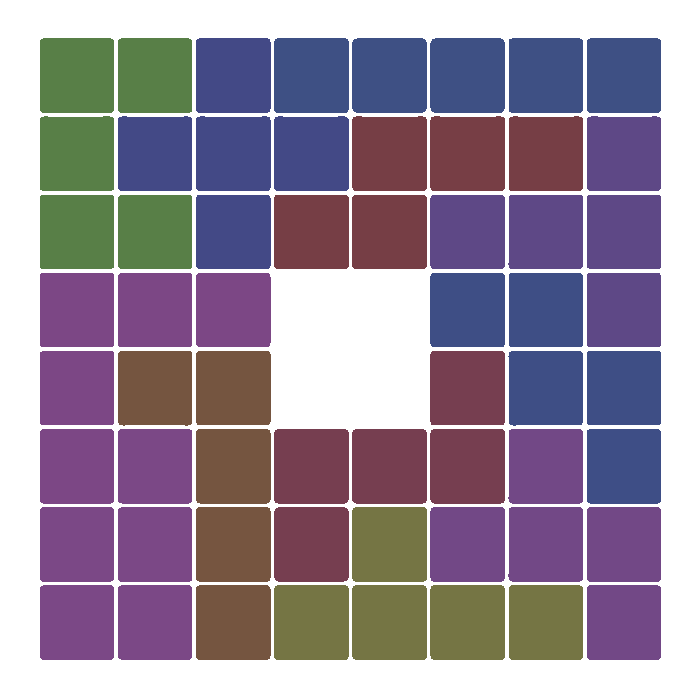
\includegraphics[height=10cm]{pavage}
\caption{Affichage d'une des solutions du problème de Scott calculée par le programme}
\end{figure}

\begin{thebibliography}{9}
\bibitem{Knuth} Donald E. Knuth. \emph{Dancing links. Millenial Perspectives in Computer Science}, 2000.
\url{http://arxiv.org/abs/cs/0011047}.
\end{thebibliography}



\end{document}